%This template consists of the minimum of a single book.
%Please do not think this template is mandatory and the format must be followed strictly.
%We expect the author adds what he needs.
\documentclass[oneside,11pt,pdftex]{book}%Remove draft when book editing is completed.
\usepackage{graphicx}
\usepackage{amsmath}
%\usepackage{fontawesome5}
\usepackage{booktabs}
\usepackage{amssymb}	
\usepackage{longtable}
\usepackage{amsthm}
\usepackage{multirow}
\usepackage[activate={true,nocompatibility},final,tracking=true,kerning=true,spacing=true,factor=1100,stretch=10,shrink=10]{microtype}
\usepackage[toc,page]{appendix}
\usepackage[nottoc]{tocbibind}
\numberwithin{equation}{section}
\graphicspath{ {./Images/} }
%\usepackage[raggedright]{titlesec}
\usepackage{placeins}
\usepackage{mathtools}


\usepackage{fancyhdr}
\usepackage{hyperref}
%Be careful when you use commands which align formulas.
%If aligned formulas range to two pages, the formulas should be divided into two environments.
%\makeatletter
%\AtBeginDocument{\let\mathaccentV\AMS@mathaccentV}
%\makeatother
%This is a patch for double bar.
%Activate it if \bar{\bar{a}} doesn't work.

\newskip\thskip
\thskip=0.5\baselineskip plus 0.2\baselineskip minus 0.2\baselineskip

\newdimen\dtest%Remove this when book editing is completed.
\settowidth{\dtest}{letters and symbols here}
\typeout{<<<\the\dtest>>>}

\newtheorem{theorem}{Theorem}[chapter]%Modify these declarations for your need.
\newtheorem{lemma}[theorem]{Lemma}
\newtheorem{corollary}[theorem]{Corollary}
\newtheorem{example}[theorem]{Example}
\newtheorem{definition}[theorem]{Definition}

\newtheorem{xca}[theorem]{Exercise}

\newtheorem{remark}[theorem]{Remark}

\numberwithin{section}{chapter}
\numberwithin{equation}{chapter}

\makeindex

\newcommand{\R}{\mathbb{R}}
\newcommand{\Q}{\mathbb{Q}}
\newcommand{\C}{\mathbb{C}}
\newcommand{\Z}{\mathbb{Z}}
\newcommand{\N}{\mathbb{N}}
\newcommand{\D}{\mathbb{D}}
\newcommand{\F}{\mathbb{F}}

\graphicspath{ {graphics/} }

\begin{document}


\frontmatter

\thispagestyle{empty}
\begin{flushright}
{\LARGE \textbf{Bhoris Dhanjal}}%Input your name here.
\end{flushright}
\vfill
\begin{center}
{\fontsize{29.86truept}{0truept}\selectfont \textbf{Probability and Sampling Distributions (B)}}%Input the book title here.
%Below is for a book with a subtitle.
%{\fontsize{29.86truept}{0truept}\selectfont \textbf{The Book Title}} \\
%\vspace{6.5truept}
%{\Large, \LARGE, etc. \textbf{The Subtitle}}
\end{center}
\vfill
\begin{flushleft}
{\LARGE \textbf{Lecture Notes}} \\
\hspace{-1.75truept}
{\large \textbf{for SSTA401}}
\end{flushleft}
\newpage

\tableofcontents


\mainmatter

\chapter[Continuous probability distributions]{Transformation of random variables \& standard univariate continuous probability distributions}
\section{Uniform/Rectangular distributions}
\begin{definition}\label{def:uniformdist}
	A r.v. $ X$ is said to follow uniform distribution over an interval $ (a,b) $ if its pdf is constant over the entire range.
\end{definition}
\subsection{PDF of uniform distribution}
\begin{theorem}
	PDF of uniform distribution
	\begin{align*}
		P(x)&=k && a<x<b\\
		&=0 && \text{otherwise}
	\end{align*}
\end{theorem}



\begin{itemize}
	\item $ \int_a^b f(x)\, dx=\int_a^b k\, dx = k[x]_a^b=k(b-a)=1$, therefore $k= \frac{1}{b-a} $
	\item We denote it as, $ X \sim U(a,b) $
	\item $ f(x)=\frac{1}{b-a} $\\ 
\end{itemize}

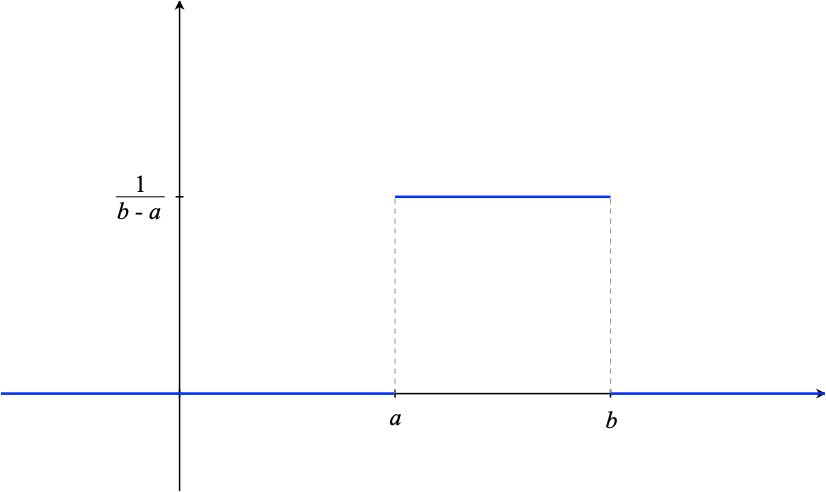
\includegraphics[scale=0.3]{uniform}

\subsection{CDF of uniform distribution}
\begin{theorem}\label{ref:cdfuniform}
	CDF of uniform distribution
	\begin{align*}
		F(x)&=0 && x \leq a\\
		&= P(X\leq x)= \int_a^x f(x)\,dx=\frac{x-a}{b-a} && a<x<b\\
			&=1 && x\geq b
	\end{align*}
\end{theorem}


\subsection{Expectation and variance of uniform distribution}
\begin{theorem}
	Expected value of $ X \sim U(a,b) $ is equal to $\frac{(a+b)}{2}$
\end{theorem}


\begin{proof}
	Consider the expectation of the uniform distribution as,
	\begin{align*}
		E[x]&=\int_a^b x P(x)\, dx\\
		&= \int_a^b x \frac{1}{b-a}\, dx\\
		&= \frac{1}{b-a} \int_a^b x\, dx\\
		&= \frac{a+b}{2}
	\end{align*}
\end{proof}

\begin{theorem}
	Variance of uniform distribution is equal to $ \frac{1}{12} (b-a)^2$
\end{theorem}
\begin{proof}
	We begin by finding out $ E[X^2] $
	\begin{align*}
		E[X^2]&=\int_a^b x^2 P(x)\, dx\\
		&= \int_a^b x^2 \frac{1}{b-a}\, dx\\
		&= \frac{1}{b-a}\int_a^b x^2\, dx\\
		&= \frac{1}{3}\left( a^2+ab+b^2\right)
\intertext{Now we can find the variance as $ V[X]=E[X^2]-E[X]^2 $ as follows,}
		V[X]&=E[X^2]-E[X]^2\\
		&= \frac{1}{3}\left( a^2+ab+b^2\right)-\left( \frac{a+b}{2}\right)^2\\
		&=\frac{(b-a)^2}{12}
	\end{align*}
\end{proof}


\subsection{Raw moments of uniform distribution}
The $ r^{th} $ raw moment of the uniform distribution is given as 

\begin{align*}
	\mu_r'&=E[X^r]=\int_a^b x^r f(x)\, dx \\
	&= \frac{1}{b-a}\left[ \frac{x^{r+1}}{r+1} \right]_a^b=\frac{b^{r+1}-a^{r+1}}{(b-a)(r+1)}
\end{align*}


\begin{example}
	Suppose in a quiz there are 30 participants. A question is given to all 30 participants and the time allowed is 25 seconds. 
\end{example}
\begin{proof}
	Let $ X$ denote the time to respond.\\
	$ X \sim U(0,25) $, the pdf is given by 
	$ f(x) =\frac{1}{25}; 0<x<25$ and $ 0 $ otherwise.
	$$ P(x\leq 6)=\int_0^6 f(x)\, dx=\int_0^6 \frac{1}{25}\, dx = \frac{151}{25}$$
	\[P(6 \leq x \leq 10)=\int_6^10 f(x)\, dx = \int_6^{10} \frac{1}{25}\, dx= \frac{101}{25} \]
\end{proof}

\begin{example}
	A r.v. $ x $ is said to follow uniform dist with $ \mu=1 $ and $ V(x) = 4/3$. Obtain $ P(x<0) $.
\end{example}
\begin{proof}
	First begin by finding out the parameters for the unfirom distribution.\\
	First consider the mean,
	\begin{align*}
		\mu&=1\\
		\frac{a+b}{2}&=1\\
		a+b&=2
	\end{align*}
	Then consider the variance,
	\begin{align*}
		V(x)&=\frac{4}{3}\\
		\frac{(b-a)^2}{12}&=\frac{4}{3}\\
		(b-a)^2&=16
	\end{align*}
	Solving two simultaneous equations we get $ a=-1, b=3 $.\\
	Therefore, we have $ X \sim U(-1,3) $\\
	\begin{align*}
		P(x\leq0)&=F(0)=\frac{0+1}{4}=\frac{1}{4}
	\end{align*}
\end{proof}


\begin{example}
	If $ X \sim U(-3,3) $, find $ P(x<2) $, $ P(|x|<2) $, $ P(|x-2|<2),$ also obtain $ k $ if $ P(x>k) =1/3$
\end{example}
\begin{proof}
	\begin{align*}
		P(x<2)&=F(2)=\frac{2+3}{6}=
		\frac{5}{6}\\
		P(|x|<2)&=\int_-2^2 \frac{1}{6}\, dx = \frac{2}{3}\\
		P(|x-2|<2)&=\int_0^3 \frac{1}{6}=\frac{1}{2}\\
		P(x>k)=1/3\implies \dots
	\end{align*}
	Complete this l8r alig8r
	
\end{proof}

\subsection{MGF of Uniform distribution}
\begin{theorem}
	MGF of Uniform distribution  $= \frac{e^{bt}-e^{at}}{t(b-a)}, t\neq0 $ and $ =1, t=0 $
\end{theorem}
\begin{proof}
	\begin{align*}
		M_x(t)&=E[e^{tx}]=\int_a^b \frac{e^{tx}}{b-a}\, dt= \frac{e^{bt}-e^{at}}{(b-a)t}
		\intertext{The Taylor series for this can be expressed as the following,}
		M_x(t)&=\frac{b-a}{b-a}+\frac{b^2-a^2}{2(b-a)}t+\frac{b^3-a^3}{3(b-a)}\frac{t^2}{2!}+\cdots
	\end{align*}
	Therefore we can say, 
	\begin{align*}
		 \mu_1'&= \text{coeff of } t=\frac{b^2-a^2}{2(b-a)}=\frac{a+b}{2}\\
		 \mu_2'&= \text{coeff of }\frac{t^2}{2!}=\frac{b^3-a^3}{3(b-a)}
	\end{align*}
And we can say $ \mu_2 = \dots$ 
\end{proof}

\subsection{Applications of uniform distribution}
\begin{enumerate}
	\item Assumption of uniform death for insurance\\
    $ \vdots $
\end{enumerate}
Write sumthin here

\section{Gamma distribution}
\begin{definition}[Gamma distribution]
	A r.v. $ `X' $ is said to follow gamma distribution $ X \sim G(\lambda, \theta) $. Where $ \lambda=$ shape parameter and $ \theta= $ scale parameter.
\end{definition}

\subsection{PDF of Gamma distribution}
\begin{definition}[PDF of Gamma distribution]
	\begin{align*}
		f(x,\lambda, \theta)&=\frac{\theta^{\lambda}}{\Gamma (\lambda)} e^{-\theta x} x^{\lambda -1}&& x>0, \lambda>0, \theta>0\\
		&= 0 && \text{otherwise}
	\end{align*}
Where $ \Gamma (\lambda)=(\lambda-1)!=(\lambda-1)\Gamma (\lambda -1) $.\\
\end{definition}





\begin{corollary}
	If $ \theta=1 $ we will have gamma distribution with a single parameter $ \lambda $ which is called the standard gamma distribution.
	\begin{align*}
		X\sim G(\lambda)&= \frac{e^{-x} x^{\lambda -1}}{\Gamma (\lambda )} && x>0, \lambda >0\\
		&=0 && \text{otherwise}
	\end{align*}
\end{corollary}

\begin{corollary}
	If $ \lambda=1, X \sim G(1, \theta) = \text{Exp}(\theta)$.
\end{corollary}

\begin{corollary}
	If $ \lambda=1, \theta=1 $, $ X \sim  $ Standard exponential distribution, i.e.
	\begin{align*}
		f(x)&= e^{-x} && x>0\\
		&=0 && \text{otherwise}
	\end{align*}
\end{corollary}


\begin{definition}[Gamma function]
	\[ \Gamma(\lambda) =\int_0^\infty e^{-x} x^{\lambda -1 }\, dx \]
\end{definition}

\begin{definition}[Gamma integral]
	\[ \int_0^\infty e^{- \theta x} x^{\lambda -1}\, dx = \frac{\Gamma (\lambda)}{\theta^\lambda}\]
\end{definition}

\subsection{CDF of Gamma distribution}
\begin{theorem}
 	CDF of Gamma distribution is given as \[ F(x) = \]
\end{theorem}
\begin{proof}
	\begin{align*}
		F(x)&=P(X<x)=\int_0^x \frac{\theta ^\lambda e^{- \theta x} x^{\lambda -1}}{\Gamma (\lambda )}\, dx\\
		&=\frac{\theta^{\lambda}}{\Gamma(\lambda)} \int_0^x x^{\lambda-1} e^{-\theta x}\, dx
	\end{align*}
\end{proof}

\subsection{Raw moments of Gamma distribution}
\begin{theorem}
	The $ r^{th} $ raw moment of the Gamma distribution is given by \[\mu_r'=\frac{\Gamma(\lambda+r)}{\Gamma(\lambda)\theta^r} \]
\end{theorem}
\begin{proof}
	\begin{align*}
		\mu_r'=E[x^r]&=\int_0^\infty \frac{x^r \theta^\lambda e^{-\theta x} x^{\lambda -1}}{\Gamma(\lambda)}\, dx\\
		&=\int_0^{\infty} \dfrac{\theta^{\lambda} e^{-\theta x}x^{\lambda+r-1}  }{\Gamma(\lambda)}\, dx\\
		&= \frac{\Gamma(\lambda+r)}{\Gamma(\lambda) \theta^r}
	\end{align*}
\end{proof}

\subsection{Mean and Variance of Gamma distribution}
Now we can find $ \mu_1', \mu_2' $
\begin{align*}
	E[x]= \mu_1'&=\frac{\lambda}{\theta}\\
	\mu_2'&= \frac{\lambda(\lambda+1)}{\theta^2}\\
	V[x] = \mu_2 &=\mu_2'-\mu_1'^2=\frac{\lambda(\lambda +1)}{\theta^2}-\frac{\lambda^2}{\theta^2}=\frac{\lambda}{\theta^2}
\end{align*}

\subsection{MGF of Gamma distribution}
\begin{align*}
	 E[e^{tx}]&=\int_0^{\infty} e^{tx} \frac{\theta^\lambda e^{-\theta x} x^{\lambda -1}}{\Gamma(\lambda )}\, dx\\
	 &= \frac{\theta^{\lambda}}{\Gamma (\lambda)} \int_0^{\infty} e^{-(\theta - t) x}x^{\lambda -1}\, dx\\
	 &= \frac{\theta^\lambda}{\Gamma(\lambda )} \frac{\Gamma(\lambda )}{(\theta -t )^{\lambda}}=\left( \frac{\theta}{\theta - t}\right)^\lambda\\
	 &=\left(1- \frac{t}{\theta}\right)^{- \lambda}
\end{align*}

\subsection{CGF of Gamma distribution}
\begin{align*}
	K_x(t)&=\log \left( 1- \frac{t}{\theta} \right)^{-\lambda}\\
	&= -\lambda \log \left(1- \frac{t}{\theta}\right)\\
	&= \frac{\lambda t }{\theta }+\frac{\lambda t^2}{2 \theta^2}+\frac{\lambda t^3}{3 \theta^3}+ \cdots
\end{align*}
Using this we can get the mean and variance easily.
\begin{align*}
	\text{Mean }&=k_1=\frac{\lambda }{\theta}\\
	\text{Variance }&= k_2= \frac{\lambda }{\theta^2}
	\end{align*}

\subsection{Additive property of Gamma distribution}
If $ X_i (i=1,\dots, k) $ are $ k $ independent Gamma distributions with parameters $ \lambda_1, \lambda_2, \dots, \lambda_k  $ and $ \theta  $ respectively, then,
\begin{align*}
	\sum_{i=1}^{k}X_i &\sim G \left( \sum_{i=1}^{k} \lambda_i, \theta \right)\\
	M_{X_i}(t)&= \left(1 -\frac{t}{\theta} \right)^{-\lambda_i}
	\intertext{Let $ Z=\sum X_i $}
	M_Z(t)&= \prod_{i=1}^k \left(1- \frac{t}{\theta}\right)^{-\lambda_i}\\
	&= \left(1- \frac{t}{\theta}\right)^{- \sum \lambda_i}
	\intertext{By uniqueness property of mgf}
	\sum_i X_i &\sim G \left(\sum_i \lambda_i, \theta \right)
\end{align*}

\subsection{Limiting form of Gamma distribution}
\begin{align*}
	\beta_1 &= \frac{4}{\lambda}, \text{ as $ \lambda \rightarrow \infty $}, \beta_1 \rightarrow 0 \implies \text{Normal dist}\\
	\beta_2 &= 3+ \frac{6}{\lambda } \text{ as $ \lambda \rightarrow \infty $}, \beta_2 \rightarrow 3 \implies \text{Normal dist}
\end{align*}
Note that they are both independent of $ \theta  $.\\
Therefore, as $ \lambda \rightarrow \infty  $ we have $ G(\lambda , \infty ) \rightarrow N \left(\frac{\lambda}{\theta}, \frac{\lambda }{\theta^2}\right)$.

\subsection{Applications of Gamma distribution}
Idk write something bruh

\section{Exponential distribution}
\subsection{PDF of Exponential Distribution}
\begin{definition}[PDF of Exponential distribution]
	A r.v. $ x $ is said to follow the exponential distribution with parameter $ \theta  $ if its pdf is given by 
	\begin{align*}
		f(x)&= \theta e^{-\theta x} && x\geq 0, \theta > 0\\
		&= 0 && \text{otherwise}
	\end{align*}
\end{definition}


\subsection{INCOMPLETE CDF of exponential distribution}
\begin{align*}
	F[x]=1-e^{-\theta x}
\end{align*}
\textbf{FILL THIS UP}
\subsection{Raw moment of exponential distribution}

\begin{theorem}
	The $ r^{th} $ raw moment for exponential distribution is given by \[ \mu_r'=\frac{r!}{\theta^r} \]
\end{theorem}
\begin{proof}
	\begin{align*}
		\mu_r'=E[x^r]&=\int_0^\infty x^r \theta e^{-\theta x}\, dx\\
		&=\frac{\Gamma(r+1)}{\theta^r}\\
		&= \frac{r!}{\theta^r}
	\end{align*}
\end{proof}

\subsection{Mean and variance of exponential distribution}
\begin{theorem}
	The mean of exponential distribution is given be \[ \mu=\frac{1}{\theta} \]
\end{theorem}
\begin{proof}
	Consider $ r=1 $,
	\begin{align*}
		\mu_1'=\frac{1}{\theta}
	\end{align*}
\end{proof}

\begin{theorem}
	The variance of the exponential distribution is given by \[ \mu_2 = \frac{1}{\theta^2}\]
\end{theorem}
\begin{proof}
	First find $ \mu_2' $
	\begin{align*}
		\mu_2'=\frac{2}{\theta^2}
	\end{align*}
So now we can compute the variance as $ \frac{1}{\theta^2} $
\end{proof}

\subsection{MGF of exponential distribution}
\begin{theorem}
	MGF of exponential distribution is given by \[ M_x(t)= \left(1- \frac{t}{\theta}\right)^{-1} \]
\end{theorem}
\begin{proof}
	\begin{align*}
		M_x(t)&=E[e^{tx}]\\
		&=\int_0^\infty e^{tx} \theta e^{-\theta x}\, dx\\
		&=\theta \int_0^\infty e^{x(t-\theta)} x^{1-1}\, dx\\
		&= \frac{\theta \Gamma(1)}{\theta - t}\\
		&=\frac{\theta }{\theta-t}\\
		&= \left(1- \frac{t}{\theta}\right)^{-1}
	\end{align*}
\end{proof}

\subsection{CGF of exponential distribution}
\begin{theorem}
	CGF of exponential distribution is given by \[ K_x(t)=-\log\left(1- \frac{t}{\theta}\right) \]
\end{theorem}
\begin{proof}
	\begin{align*}
		K_x(t)&= \log \left(1-\frac{t}{\theta}\right)^{-1}\\
		&= -\log\left(1- \frac{t}{\theta}\right)\\
		&= \frac{t}{\theta }+\frac{t^2}{2 \theta^2}+\frac{t^3}{3 \theta^3}
	\end{align*}
We can say the general $ r^{th} $ cumulant is given by $ K_r=\frac{(r-1)!}{\theta^r} $
\end{proof}

\subsection{Additive property of exponential variates}
\begin{theorem}
	If $ x_1,x_2,\dots,x_k $ are $ k $ independent exponential variates each with parameter $ \theta  $then \[ \sum_{i=1}^k x_i \sim G(k, \theta)\]
\end{theorem}
\begin{proof}
	We will do this with the MGF. Consider taht $ Z=\sum{i=1}^{k} x_i $.
	\begin{align*}
		M_z(t)&=\prod_{i=1}^{k} M_x(t)\\
		&= \prod_{i=1}^k \left(1- \frac{t}{\theta}\right)^{-1}\\
		&= \left(1- \frac{t}{\theta}\right)^{-k}
	\end{align*}
Therefore, (by uniqueness property of MGF) comparing this MGF to that of the gamma distribution we can say that,
$$ \sum_{i=1}^k x_i = Z \sim G(k,\theta)$$
\end{proof}

\subsection{Lack of memory of exponential distribution}
\begin{theorem}
	For a exponentially distributed random variate, $ P[x>a+b \mid x>a]=P[x>b] $
\end{theorem}
\begin{proof}
	Let $ X \sim E(\theta) $. Consider first case
	\begin{align*}
		P[x>a+b \mid x>a]&= \frac{P[x>a+b]}{P[x>a]}\\
		&=\frac{\int_{a+b}^\infty \theta e^{-\theta x}\, dx}{\int_a^\infty \theta e^{-\theta x}\, dx}\\
		&=\frac{e^{-\theta a+b}}{e^{-\theta a}}\\
		&=e^{-\theta b}
	\end{align*}
	Consider second case now,
	\begin{align*}
		P[x>b]&=\int_b^{\infty }\theta e^{-\theta x}\, dx=e^{-\theta b}
	\end{align*}
	Equality holds.
\end{proof}

\section{INCOMPLETE Laplace distribution (Double exponential)}
\subsection{PDF}
\begin{definition}[PDF of Laplace distribution]
	$ X\sim L (\lambda, \mu)$\[ f(x)=\begin{cases}
		\frac{1}{2 \lambda } e^{-\left|\frac{x-\mu }{\lambda}\right|} & -\infty<x<\infty\\
		0 & \text{otherwise}
	\end{cases} \]
\end{definition}
\subsection{CDF}
\begin{definition}[CDF of Laplace distribution]
	\[ F[x]=\begin{cases}
		content...
	\end{cases} \]
\end{definition}

\subsection{Raw moment}
\begin{theorem}
	The $ r^{th} $ raw moment for the Laplace distribution is given by \[ \mu_r'= \]
\end{theorem}
\begin{proof}
	\begin{align*}
		\mu_r'&=E[x^r]=\int_{-\infty}^\infty \frac{x^r}{2 \lambda }e^{-\left|\frac{x-\mu }{\lambda}\, dx\right|}
		\intertext{Transform $ (x-\mu)/\lambda =z $}
		&=\frac{1}{2\lambda }\left( \int_{-\infty}^\infty (z\lambda+\mu)^r e^{-|z|}\, \lambda\, dz  \right)\\
		&=\frac{1}{2} \left(\int_{-\infty}^\infty \sum_{k=0}^{r}\binom{r}{k} (z-\lambda)^k \mu^{r-k} e^{-|z| \, dz}\right)\\
		&=\frac{1}{2}\sum_{k=0}^r \left[\binom{r}{k}\lambda^k \mu^{r-k} \int_{-\infty}^\infty z^k e^{-|z|}\, dz \right]\\
		\intertext{Complete this up}
		&=\frac{1}{2}\sum_{k=0}^{r} \left[\binom{r}{k} \lambda^k \mu^{r-k} k! (1+(-1)^k)\right]
	\end{align*}
\end{proof}

\subsection{Mean and variance}
We can do this with the raw moments above but instead we will do it with the PDF.
\begin{theorem}
	Expectation of laplace distribution is given as \[ E[x]= \]
\end{theorem}
\begin{proof}
	\begin{align*}
		E[x]&=\int_{-\infty }^{\infty }x f(x)\, dx\\
		&=\int_{-\infty }^{\infty }\frac{x}{2\lambda}e^{-\left|\frac{x-\mu }{\lambda}\right|}\, dx
		\intertext{Split it around $ \mu $}
		&=\frac{1}{2\lambda}\left( \int_{-\infty}^\mu x e^{\frac{x-\mu }{\lambda}}\, dx + \int_\mu^{\infty}x e^{-\frac{x-\mu }{\lambda}}\, dx \right)\\
		&= \frac{1}{2\lambda} \left[ e^{-\mu/ \lambda}\int_{-\infty}^{\mu} xe^{x/\lambda}\, dx + e^{\mu/\lambda}\int_{\mu}^{\infty}xe^{-x/\lambda}\, dz\right]\\
		&=\frac{1}{2 \lambda} \left[e^{-\mu/\lambda } \lambda(x-\lambda)e^{x/ \lambda}-e^{\mu/\lambda }(\lambda(x+\lambda)e^{-x/ \lambda}) \right]\\
		&=\mu
	\end{align*}
\end{proof}

\begin{theorem}
	Expectation of $ x^2 $ in Laplace distribution is given be \[ E[x^2]=bruh \]
\end{theorem}
\begin{proof}
	\begin{align*}
		E[x^2]&=\int_{-\infty}^\infty x^2 \frac{1}{2\lambda }e^{-\left| \frac{x-\mu }{\lambda} \right|}
		\intertext{Split it around $ \mu $}
		&=\frac{1}{2\lambda}\left( \int_{-\infty}^\mu x^2 e^{\frac{x-\mu }{\lambda}}\, dx + \int_\mu^{\infty}x^2 e^{-\frac{x-\mu }{\lambda}}\, dx \right)\\
		&= \frac{1}{2\lambda} \left[ e^{-\mu/ \lambda}\int_{-\infty}^{\mu} x^2e^{x/\lambda}\, dx + e^{\mu/\lambda}\int_{\mu}^{\infty}x^2e^{-x/\lambda}\, dx\right]\\
		&= \frac{1}{2\lambda} \left[ e^{-\mu/ \lambda}(\lambda (x^2-2\lambda x+2\lambda^2)e^{x/\lambda}) - e^{\mu/\lambda}(\lambda(x^2+2\lambda x+2\lambda^2)e^{-x/ \lambda})\right]\\
		&=2\lambda^2
	\end{align*}
\end{proof}
\begin{theorem}
	Variance of Laplace distribution is given as \[ V[x]= \]
\end{theorem}


\subsection{MGF}
\begin{theorem}
	MGF of the Laplace distribution is given by \[ M_x(t)=bruh \]
\end{theorem}
\begin{proof}
	\begin{align*}
		M_x(t)&=E[e^{tx}]=\int_{-\infty}^\infty \frac{1}{2\lambda} e^{tx-\left|\frac{x-\mu }{\lambda}\right|}\\
		&=\frac{1}{2\lambda}\left[e^{-\mu/\lambda} \int_{-\infty}^\mu e^{x\left(t+\frac{1}{\lambda} \right)}\, dx + e^{\mu/\lambda}\int_\mu^{\infty} e^{-x\left(\frac{1}{\lambda}-t \right)}\, dx\right]\\
		&= \frac{1}{2 \lambda } \left[e^{-\mu/\lambda} \left(\frac{e^{\mu \left( \frac{1}{\lambda} +t \right)}}{\frac{1}{\lambda}+t}\right) + e^{\mu/\lambda} \left(\frac{-e^{\mu \left(\frac{1}{\lambda}-t \right)}}{-\frac{1}{\lambda} +t}\right)\right]\\
		&=\frac{1}{2\lambda }\left[\frac{e^{\mu t}}{t+\frac{1}{\lambda}}-\frac{e^{\mu t}}{t-\frac{1}{\lambda}}\right]
	\end{align*}
\end{proof}

Plot a graph for the beta-1 dsitribution when alpha=5, beta=2
\subsection{CGF}

\section{Beta distribution of Type-I}
\subsection{PDF}
\begin{definition}[PDF of Beta I]
	\[ f(x)=\begin{cases}
		\frac{1}{\beta(m,n)}x^{m-1}(1-x)^{n-1} & 0<x<1; m,n>0\\
		0 & \text{otherwise}
	\end{cases} \]
	Where $ \beta(m,n) = \frac{\Gamma(m)\Gamma(n)}{\Gamma(m+n)}$
\end{definition}
Note the following,
\begin{enumerate}
	\item We can say, $ X \sim \beta_1 (m,n) $ where $ m,n $ are the parameters of the distribution.
	\item Since $ f(x) $ is a pdf we have the following,
	\begin{align*}
		\int_0^1 f(x)\, dx &= \int_0^1 \frac{1}{\beta(m,n)} x^{m-1} (1-x)^{n-1}\, dx\\
		&= \int_0^1 
	\end{align*}
\end{enumerate}

\subsection{Raw moments}
\begin{theorem}
	The $ r^{th}$ raw moment of the Beta I distribution is given by \[ \mu_r'=\frac{\Gamma(m+n)\Gamma(r+m)}{\Gamma(m)\Gamma(m+n+r)} \]
\end{theorem}
\begin{proof}
	\begin{align*}
		\mu_{r}'=E[x^r]&=\int_0^1 \frac{1}{\beta(m,n)} x^{r+m-1}(1-x)^{n-1}\, dx\\
		&=\frac{\Gamma(m+n)\Gamma(r+m)}{\Gamma(m)\Gamma(m+n+r)}
	\end{align*}
\end{proof}

\subsection{Mean and Variance}
\begin{theorem}
	Mean of Beta I distribution is given by \[ E[x]=\frac{m}{m+n} \]
\end{theorem}
\begin{proof}
	\begin{align*}
		E[x]=\mu_1'=\frac{\Gamma(m+n)\Gamma(m+1)}{\Gamma(m)+\Gamma(m+n+1)}=\frac{m}{m+n}
	\end{align*}
\end{proof}

\begin{theorem}
	Variance of Beta I distribution is given by \[ V[x]=\frac{mn}{(m+n)^2(m+n+1)} \]
\end{theorem}
\begin{proof}
	\begin{align*}
		\mu_2'&=\frac{(m+1)(m)}{(m+n)(m+n+1)}
	\end{align*}
So now we have the variance given as,
\begin{align*}
	\mu_2&=\mu_2'-\mu_1'^2\\
	&=\frac{mn}{(m+n)^2(m+n+1)}
\end{align*}
\end{proof}

\section{Beta distribution of Type-II}
\subsection{PDF}
\begin{definition}[PDF of Beta-II distribution]
	\[ f(x)=\begin{cases}
		\frac{1}{\beta(m,n)}\frac{x^{m-1}}{(1+x)^{m+n}} & 0<x<\infty; m,n>0\\
		0 & \text{otherwise}
	\end{cases} \]
\end{definition}
Note the following,
\begin{enumerate}
	\item $ X $ is said to follow $ \beta_2(m,n) $ as $ X \sim \beta_2(m,n) $
	\item \begin{align*}
		\int_0^{\infty }f(x)\, dx&=\int_0^\infty \frac{x^{m+1}}{(1+x)^{m+n}}=\beta(m,n)
	\end{align*}
\end{enumerate}

\subsection{Raw moments}
\begin{theorem}[Raw moments of Beta-2 distribution]
	The raw moments of the Beta-2 distribution is given by \[ \mu_r'= \frac{\Gamma(m+r)\Gamma(n-r)}{\Gamma(m)\Gamma(n)} \]
\end{theorem}
\begin{proof}
	\begin{align*}
		\mu_r'&=E[x^r]=\int_0^{\infty} \frac{1}{\beta(m,n)}\frac{x^{m+r-1}}{(1+x)^{m+n}}\, dx\\
		&=\frac{\Gamma(m+r)\Gamma(n-r)}{\Gamma(m)\Gamma(n)}
	\end{align*}
\end{proof}

\subsection{Mean and variance}
\begin{theorem}[Mean of Beta-2 distribution]
	The mean of Beta-2 distribution is given by \[ E[x]=\frac{m}{n-1} \]
\end{theorem}
\begin{proof}
	\begin{align*}
		E[x]&=\mu_1'=\frac{\Gamma(m+1)\Gamma(n-1)}{\Gamma(m)\Gamma(n)}\\
		&=\frac{m}{n-1}
	\end{align*}
\end{proof}

\begin{theorem}[Variance of Beta-2 distribution]
	The variance of Beta-2 distribution is given by \[ V[x]=\frac{m(m+n-1)}{(n-2)(n-1)^2} \]
\end{theorem}
\begin{proof}
	First consider the 2nd raw moment,
	\begin{align*}
		\mu_2'&=\frac{m(m+1)}{(n-2)(n-2)}
	\end{align*}
	Now we can compute the variance as follows
	\begin{align*}
		V[x]&=\mu_2=\mu_2'-\mu_1'^2=\frac{m(m+n-1)}{(n-2)(n-1)^2}
	\end{align*}
\end{proof}

\section{Transformation of variables}
\subsection{One dimensional random variable}
Let $ X $ be a continuous random variable with pdf $ f(x) $ and let $ Y=g(x) $ be a strictly monotonic function of $ X $ with unique inverse.\\
Assume that $ g(x) $ is differentiable and is continuous for all $ x $, then the pdf of r.v. $ Y $ is given by 
\[ h(y)=f(x) \cdot \det \left|\frac{dx}{dy}\right| = \left|\frac{dx}{dy}\right|\]
where r.v. $ x $ is expressed in terms of $ y $.
Steps to solve,
\begin{enumerate}
	\item Write pdf of r.v. $ X $.
	\item Express old variable $ X $ in terms of new variable $ Y $.
	\item Write the range of the new variable.
	\item Obtain $ J $ where $ J=\left|\frac{dx}{dy}\right| $ and $ |J| $.
	\item Obtain $ h(y) =f(x)\cdot |J|,$ where $ X $ is expressed in terms of $ Y. $
\end{enumerate}
\begin{remark}
		For $ 2-1 $ correspondence, i.e. for ever 2 values of $ X $ is there is only one value of $ Y $, then multiple $ |J| $ with 2.
\end{remark}
\begin{remark}
	\item For $ 1-2 $ correspondence i.e., for every 1 value of x if there are 2 values of $ Y $ then multiply $|J| $ with $ \frac{1}{2} $.
\end{remark}

\begin{example}
	If a r.v. $ X \sim B_1(m,n) $ obtain the distribution of $ Y=1-X $.
\end{example}
\begin{proof}
	First begin by stating the pdf of $ X $.
	\begin{align*}
		f(x)=\begin{cases}
			\frac{1}{\beta(m,n)}x^{m-1}(1-x)^{n-1} & 0<x<1; m,n>0\\
			0 & \text{otherwise}
		\end{cases} 
	\end{align*}
	Now $ X=1-Y $ this ranges from $ 1-Y=0 $ to $ 1-Y=1 $. So $ 0<Y<1 $ again.\\
	Now compute $ J $
	\begin{align*}
		\frac{dx}{dy}&=\frac{1}{dy} \left( 1-y \right)\\
		J&=-1\\
		|J|&=1
	\end{align*}
	We multiply this with $ f(x) $ to get $ h(y) $.
	\begin{align*}
		h(y)&=f(x)\cdot |J|\\
		h(y)&= f(x)
	\end{align*}
	So $ h(y)\sim B(n,m) $. The order changes.
\end{proof}

\begin{example}
	A r.v. $ X\sim B_2(m,n) $. Obtain the distribution of $ Y $ where $ Y=\frac{1}{1+X} $.
\end{example}
\begin{proof}
	First state the pdf,
	\begin{align*}
		f(x)=\begin{cases}
			\frac{1}{\beta(m,n)}\frac{x^{m-1}}{(1+x)^{m+n}} & 0<x<\infty; m,n>0\\
			0 & \text{otherwise}
		\end{cases}
	\end{align*}
	Now state $ X $ in terms of $ Y $, we have $ X=\frac{1}{Y}-1 $. \\
	Compute the new ranges now we have $ \frac{1}{Y}-1=0 $ so $ Y=1 $ as one side then $  \frac{1}{Y}-1=\lim_{m \rightarrow \infty} m $ so to $ Y=0 $.\\
	The new ranges are $ 0<Y<1 $.
	Now compute $ |J| $,
	\begin{align*}
		J&=\frac{dx}{dy}= \frac{1}{dy}\left( \frac{1}{y}-1 \right)\\
		&=-\frac{1}{y^2}\\
		|J|&=\frac{1}{y^2}
	\end{align*}
	So now we can compute $ h(y) $ as follows,
	\begin{align*}
		h(y)&=f(x)|J|\\
		&= \frac{1}{\beta(m,n)}\frac{\left( \frac{1}{y}-1\right)^{m-1}}{(1/y)^{m+n}}\frac{1}{y^2}\\
		&=\frac{1}{\beta(m,n)}y^{n-1}(1-y)^{m-1}
	\end{align*}
	This is for the range we have and $ 0 $ otherwise. But I'm too lazy to typeset that out as a cases.\\
	So we now have $ Y \sim B_1(n,m) $.
\end{proof}

\section{Two dimensional r.v.}
Let $ X $ and $ Y $ be two continuous independent r.v. with joint pdf $ f(x,y) $. Say $ U=g(x,y) $ and $ V=h(x,y) $ are two other r.v. then the joint pdf of $ U $ and $ V $ is given by,
\[ k(u,v)=f(x,y)\cdot |J| \]
where $ X, Y$ are expressed in terms of $ U,V $.
Here we have the Jacobian as follows,
\begin{align*}
	\begin{bmatrix}
	\frac{\partial x }{\partial u} & \frac{\partial x}{\partial v}\\[1ex]
	\frac{\partial u}{\partial u} & \frac{\partial y}{\partial v}
\end{bmatrix}=	\begin{bmatrix}
		\frac{\partial x }{\partial u} & \frac{\partial y}{\partial u}\\[1ex]
		\frac{\partial x}{\partial v} & \frac{\partial y}{\partial u}
	\end{bmatrix}
\end{align*}
\subsection{Steps to solve}
\begin{enumerate}
	\item Write the pdf of $ X $ and $ Y $, i.e. $ f(x,y) $.
	\item Express old variable in terms of new variable.
	\item Obtain range of the new variable.
	\item Obtain $ J $ and $ |J| $.
	\item Obtain $ k(u,v)=f(x,y)|J| $.
\end{enumerate}

\begin{example}
	$ X $ and $ Y $ are two independent gamma variates with parameters $ a $ and $ b $ respectively.
	\begin{enumerate}
		\item Obtain the joint distribution of $ u $ and $ v $ where $ u=x+y, v= \frac{x}{x+y} $.
		\item Show that $ u, v $ are independent and identify their distributions.
	\end{enumerate}
\end{example}
\begin{proof}
	Consider the pdf of gamma function as follows,
	\begin{align*}
		X\sim G(\lambda)&= \frac{e^{-x} x^{\lambda -1}}{\Gamma (\lambda )} && x>0, \lambda >0\\
		&=0 && \text{otherwise}
	\end{align*}
	Where $ \Gamma (\lambda)=(\lambda-1)!=(\lambda-1)\Gamma (\lambda -1) $.\\
	\begin{align*}
		f_1(x)&=\frac{1}{\Gamma (a)}e^{-x}x^{a-1}\\
		f_2(x)&=\frac{1}{\Gamma (b)}e^{-x}x^{b-1}
	\end{align*}
	Find $ f(x,y)=f_1(x)f_2(y) $
		\begin{align*}
			f(x,y)&=\frac{1}{\Gamma(a)\Gamma(b)}e^{-x-y}x^{a-1}x^{b-1} && x,y,a,b,>0\\
			&= 0 && \text{otherwise}
		\end{align*}		
	We now have the new variables $ U,V $
	$ U=X+Y, V=\frac{X}{X+Y} $. This implies that $ X=UV, Y=U(1-V)$.\\
	We need to find the new ranges now. Since $ X,Y>0 $ we have $ U>0 $ and $ X<X+Y \implies \frac{x}{x+y}<1 \implies v<1 $. And $ 0<V<1 $.\\
	
	Find the Jacobian,
	\begin{align*}
		J&=\begin{bmatrix}
			v & u\\
			1-v & -u
		\end{bmatrix}=-u\\
	|J|&=u
	\end{align*}
	The joint distribution is then given as,
	\begin{align*}
			k(u,v)&=\frac{1}{\Gamma(a)\Gamma(b)}e^{-(uv+u-uv)}(uv)^{a-1}[u(1-v)]^{b-1} \cdot u\\
			&=\frac{1}{\Gamma(a)\Gamma(b)}e^{-u}u^{a-1+b-1+1} v^{a-1} (1-v)^{b-1} \times \frac{\Gamma(a+b)}{\Gamma(a+b)}\\
			&= \frac{1}{\Gamma(a+b)}e^{-u}u^{a+b-1} \times \frac{1}{\beta(a,b)}v^{a-1}(1-v)^{b-1}\\
			&=k_1(u)k_2(v)
	\end{align*}
So $ u $ and $ v $ are independent r.v. and $ U \sim G(a+b), V \sim \beta_1(a,b) $
\end{proof}

\begin{example}
	$ X $ and $ Y $ are two independent r.v. $ X \sim G(a) $ and $ Y\sim G(b) $. We have $ U=X+Y $ and $ W=\frac{X}{Y} $. Show that $ U, W $ are independent and identify the distribution.
\end{example}
\begin{proof}
	We know the following,
\begin{align*}
	f_1(x)&= \frac{e^{-x} x^{a -1}}{\Gamma (a )} && x>0, a >0\\
	&=0 && \text{otherwise}
\end{align*}
and,
\begin{align*}
	f_2(y)&= \frac{e^{-y} y^{b -1}}{\Gamma (b)} && x>0, b >0\\
	&=0 && \text{otherwise}
\end{align*}
Now the joint distribution $ f(x,y) $ is given by its product since they are independent,
\begin{align*}
	f(x,y)&=\frac{e^{-x} x^{a -1}}{\Gamma (a )} \times \frac{e^{-y} y^{b -1}}{\Gamma (b)} && x>0,y>0; a,b >0\\
	&=0 && \text{otherwise}
\end{align*}
Now we compute the new ranges $ X = \frac{UW}{W+1}$ and $ Y=\frac{U}{W+1} $.
Now when $ X=0 $ we have $ U=0, W=0 $ when $ X\rightarrow \infty $ $ U \rightarrow \infty, V \rightarrow \infty $. So we have $ U>0 $ and $ W>0 $.\\
Now compute the Jacobian as follows,
\begin{align*}
	J&= \begin{bmatrix}
		\frac{w}{1+w} & \frac{-uw}{(1+w)^2}+\frac{u}{1+w}\\
		\frac{1}{1+w} & \frac{-u}{(1+w)^2}
	\end{bmatrix}\\
	|J|&=\frac{u}{(1+w)^2}
\end{align*}
Since for 2 values of $ Y $ we get one value of $ X $ we will multiply the jacobian by 2. Now we compute $ k(u,w) $ as follows,
\begin{align*}
	k(u,w)&=f(x,y)|J|\\
	&=\frac{e^{-\frac{uw}{w+1}} \frac{uw}{w+1}^{a -1}}{\Gamma (a )} \times \frac{e^{-\frac{u}{w+1}} \frac{u}{w+1}^{b -1}}{\Gamma (b)} \times \frac{u}{(1+w)^2}\\
	&=\frac{1}{\Gamma(a+b)}e^{-u}u^{a+b-1} \times \frac{1}{\beta(a,b)}
\end{align*}
Complete this 
\end{proof}

\begin{example}
	$ X \sim N(\mu, \sigma^2) $. Obtain the distribution of $ Y=\frac{1}{2} \left( \frac{x-\mu }{\sigma}\right)^2$
\end{example}
\begin{proof}
	Begin by stating the pdf of r.v. $ X 
	$,
	\begin{align*}
		f(x)&={\displaystyle {\frac {1}{\sigma {\sqrt {2\pi }}}}e^{-{\frac {1}{2}}\left({\frac {x-\mu }{\sigma }}\right)^{2}}} && -\infty<x<\infty, \sigma>0\\
		&=0 && \text{otherwise}
	\end{align*}
	We now state $ X $ in terms of $ Y $ as follows, $ X= \mu \pm \sqrt{2} \sigma \sqrt{y}  $. Range of $ y $ is $ 0<y<\infty $. And since it is 2-1 correspondence we will multiply the Jacobian by $ 2 $.\\
	Compute the value of Jacobian first,
	\begin{align*}
		|J|=\frac{\sigma }{\sqrt{2} \sqrt{y}}
	\end{align*}
	Now compute the new function,
	\begin{align*}
		h(y)&=f(x)|J|2\\
		&={\displaystyle {\frac {1}{\sigma {\sqrt {2\pi }}}}e^{-{\frac {1}{2}}\left({\frac {x-\mu }{\sigma }}\right)^{2}}} \times \frac{\sigma }{\sqrt{2} \sqrt{y}} \times 2\\
		&=\frac{1}{\sigma \sqrt{2\pi}}e^{-y} \frac{2 \sigma}{\sqrt{2}\sqrt{y}}\\
		&= \frac{2}{\sqrt{2}\sqrt{y} \sqrt{2 \pi}}e^{-y}\\
		&= \frac{e^{-y}}{\sqrt{\pi}\sqrt{y}}\\
		&=\frac{1}{\Gamma(\frac{1}{2})}e^{-y}y^{1-\frac{1}{2}}
	\end{align*}
	So we have $ Y \sim G\left(\frac{1}{2} \right) $.
\end{proof}


\begin{example}
	\[ f(x,y)=\begin{cases}
		4xye^{-(x^2+y^2)} & x,y>0\\
		0 & \text{otherwise}
	\end{cases} \]
Prove that $ h(u)=2u^3e^{-u^2}, u>0$ where $ u=\sqrt{x^2+y^2} $ and $ v=x $.
\end{example}
\begin{proof}
	The variables we are dealing with are,
	\[ x=v, y=\sqrt{u^2-v^2}\]
	The range for $ v, u$ is $ (0,\infty) $ but $ 0<v<u<\infty $.\\
	Begin by computing the Jacobian,
	\begin{align*}
		|J|=\frac{u}{\sqrt{u^2-v^2}}
	\end{align*}
	Consider now the joint distribution with the change of variables,
	\begin{align*}
		g(u,v)&=f(x,y)|J|\\
		&=4xye^{-(x^2+y^2)} |J|\\
		&= 4(v)(\sqrt{u^2-v^2}) e^{-(v^2+u^2-v^2)}\frac{u}{\sqrt{u^2-v^2}}\\
		&=4v\sqrt{u^2-v^2} e^{-u^2}\frac{u}{\sqrt{u^2-v^2}}\\
		&=4vue^{-u^2}
		\intertext{Integrate out v}
		h(u)&=4ue^{-u^2}\int_0^u v  \, dv \\
		&=4ue^{-u^2} \frac{u^2}{2}\\
		&=2u^3e^{-u^2}
	\end{align*}
\end{proof}

\begin{example}
	\[ f(x,y)=\begin{cases}
		\frac{e^{-(x+y)}x^3y^4}{\Gamma(4)\Gamma(5)} & x,y>0\\
		0 & \text{otherwise}
	\end{cases} \]
Obtain pdf of $ u $ where $ u=\frac{x}{x+y} $ take $ v=x+y $ also obtain $ E[u],V[u] $.
\end{example}
\begin{proof}
	Consider the new variables,
	$ x=uv, y=v-uv $. The range for $v $ is $ (0,\infty) $ and for $ u $ is $ (0,1) $\\
	Compute the Jacobian,
	\begin{align*}
		|J|=v
	\end{align*}
	Compute the joint pdf,
	\begin{align*}
		g(u,v)&=f(x,y)|J|\\
		&=\frac{e^{-(x+y)}x^3y^4}{\Gamma(4)\Gamma(5)} |J|\\
		&=\frac{e^{-(uv+v-uv)}(uv)^3(v-uv)^4}{\Gamma(4)\Gamma(5)} v\\
		&= \frac{e^{-v}u^3(1-u)^{4}v^8}{\Gamma(4)\Gamma(5)}\\
		\intertext{Integrate out v}\\
		h(u)&=\frac{u^3(1-u)^{4}}{\Gamma(4)\Gamma(5)} \int_0^\infty e^{-v}v^8 \, dv\\
		&=\frac{\Gamma(9)}{\Gamma(4)\Gamma(5)}u^3 (1-u)^4\\
	\end{align*}
So $ U \sim \beta_1(m=4,n=5)$. Compute the mean and variance as follows,
\begin{align*}
	E[U]&=\frac{m}{m+n}=\frac{4}{9}\\
	V[U]&=\frac{mn}{(m+n)^2(m+n+1)}=\frac{20}{810}=\frac{2}{81}
\end{align*}
\end{proof}

\begin{example}
	$ X , Y$ are two independent gamma variates with parameters $ a,b $ respectively. Show that $ U+X+Y, V=\frac{X-Y}{X+Y} $ are independent.
\end{example}
\begin{proof}
	Consider the original pdfs,
	\begin{align*}
		f_1(x)&=\frac{e^{-x} x^{a -1}}{\Gamma (a)}\\
		f_2(y)&=\frac{e^{-y} x^{b -1}}{\Gamma (b)}
		\intertext{Since they are independent}
		f(x,y)&=\frac{e^{-(x+y)}x^{a-1}y^{b-1}}{\Gamma(a)\Gamma(b)}
	\end{align*}
	Consider the new variables,
	$ x=\frac{1}{2} (uv+u), y= \frac{1}{2}(u-uv) $, the ranges for $ u $ is $ (0,\infty) $ but for $ v $ is $ (-1,1) $\\
	Compute the Jacobian,
	\begin{align*}
		|J|=\frac{u}{2}
	\end{align*}
	Compute the joint pdf,
	\begin{align*}
		g(u,v)&=f(x,y)|J|\\
		&=\frac{e^{-(x+y)}x^{a-1}y^{b-1}}{\Gamma(a)\Gamma(b)} |J|\\
		&=-\frac{e^{-u} (v+1) 2^{-a-b+2} (u (v+1))^{a-2} (u-u v)^b}{(v-1) \Gamma (a) \Gamma (b)}
	\end{align*}
	Split this up I'm too lazy to type it.
\end{proof}


\chapter{Chi-square distribution}



\chapter{F-distribution}


\backmatter


\thispagestyle{empty}%If your book ends with the even numbered page, copy and paste it twice. With the odd numbered page, do it three times.
{\ }
\newpage

\end{document}
